\documentclass{article}
\usepackage[utf8]{inputenc}
\usepackage[T1]{fontenc}
\usepackage{graphicx}
\usepackage{hyperref}
\usepackage{geometry}
\geometry{margin=1in}

\title{LAVA and VOLCANOLOGY (Plate CCLXXIV)}
\date{Encyclopaedia Britannica (1771)}

\begin{document}
\maketitle

\section*{Historical source}
\textbf{Entry ID:} \texttt{entry-britannica-volume-149982692-row-948-948} \\
\textbf{Volume ID:} 149982692 \\
\textbf{Character Count:} 1157

\subsection*{Extracted Text}
Lava.
Plate CCLXXIV.

[HISTORICAL COPPERPLATE ENGRAVING: LAVA and VOLCANOLOGY (Plate CCLXXIV)]
Category: Geology and Mineralogy
Visual Description: Engraved natural history plate showing volcanic rock specimens, cooled basaltic lava structures, and vesicular pumice formations. Depicts columnar jointing typical of the Giant's Causeway and volcanic craters in active eruption.

[Nemotron Super VL Analysis]: This image does not depict lava or volcanology; it is Plate CCLXXIV featuring zoological illustrations of birds and invertebrates. Visible headings include "Livia," "Lepama," "Limax," "Libellula," and "Lumbricus marinus." The key figures consist of six birds labeled A through F perched on branches under "Livia," along with lower illustrations of a larva, two mollusks, a dragonfly, and a long segmented worm.
Identified Engraved Figures:
  * Fig. 1: Cross-section of volcanic crater and basaltic columnar lava flow
  * Fig. 2: Specimen of vesicular lava with mineral crystal inclusions
  * Fig. 3: Prismatic basalt columns showing hexagonal fracturing pattern
Related Scientific Subjects: Lava, Basalt, Columnar jointing, Volcanology, Igneous rock

\subsection*{Matched Wikipedia Article}
\textbf{Title:} History of the Encyclopædia Britannica \\
\textbf{Page ID:} 9004976 \\
\textbf{Revision ID:} 1340071003 \\
\textbf{URL:} \url{https://en.wikipedia.org/wiki/History\_of\_the\_Encyclop\%C3\%A6dia\_Britannica}


\section*{Source record}
\begin{itemize}
\item \textbf{Dataset:} \texttt{NationalLibraryOfScotland/encyclopaedia\_britannica\_illustrated}
\item \textbf{Dataset Revision:} \texttt{309f765b1ecc83e0a7f7762e44b4a927a7555443}
\item \textbf{Page ID:} \texttt{britannica:309f765b1ecc83e0a7f7762e44b4a927a7555443:train:948} \\
  \textbf{Filename:} \texttt{page-0948-7daaf1d3d872.jpg} \\
  \textbf{Row Index:} 948 \\
  \textbf{SHA256:} \texttt{7daaf1d3d872629a...}
\end{itemize}

\begin{figure}[h]
\centering
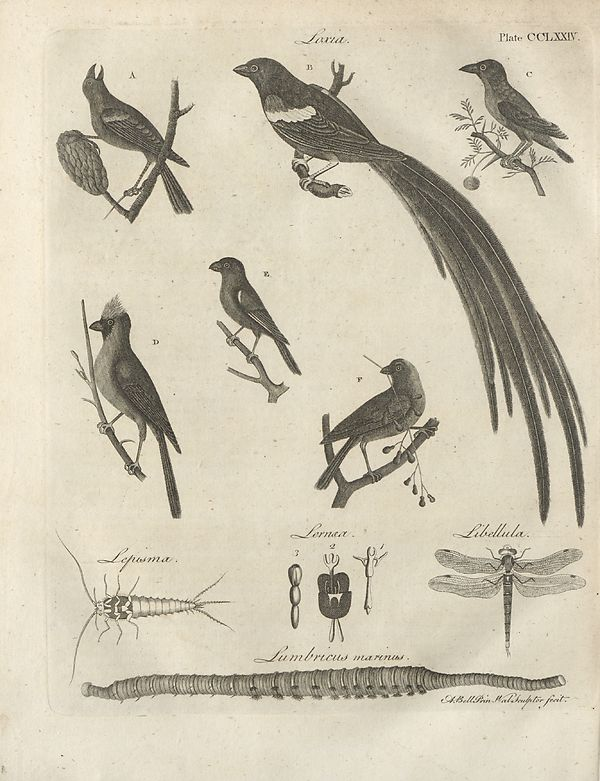
\includegraphics[width=0.85\textwidth]{../scans/page-0948-7daaf1d3d872.jpg}
\caption*{Source scan: \texttt{page-0948-7daaf1d3d872.jpg}}
\end{figure}

\end{document}
